\newpage
%**************************************************************
\chapter{The White Dog s.r.l.}
\label{cap:thewhitedog}

\section{Chi è The White Dog s.r.l.}

The White Dog s.r.l. è una realtà aziendale nata nel 2008 con sede a Torreglia, in provincia di Padova. Essa è stata fondata dal signor Stefano Mocellini, fondatore e CEO di Diana Corp. \\
The White Dog s.r.l. coordina e gestisce società tutte affini al settore e-commerce, come Diana Corp. e LiveStory. L'azienda possiede un nucleo interno denominato R\&D, il quale esplora nuove tecnologie da applicare poi alle società figlie nel caso di esito positivo o facendo nascere nuovi progetti separati.

\label{The White Dog s.r.l.}
\begin{figure}[ht]
	\begin{center}
		
\includegraphics[scale=1]{twd_logo}
		\caption{Logo dell'azienda The White Dog s.r.l.}
	\end{center}
\end{figure}
\FloatBarrier

\section{Prodotti e servizi}

Il principale servizio che l'azienda offre a Diana Corp. è la ricerca e lo sviluppo di nuove tecnologie da applicare nell'ambito del fashion e-commerce. Essa svolge l'attività di \textit{testing} delle nuove tecnologie web disponibili, le valuta attentamente in termini di prestazioni e costi, per poi renderle disponibili all'azienda Diana Corp.. Ad essa oltretutto vengono commissionati progetti che Diana Corp., per competenze e tempistiche, non può portare a termine, come ad esempio applicazioni \textit{mobile} legate agli e-commerce prodotti. \\ \\
Il prodotto cardine però dell'azienda è sicuramente \textit{Live Story}. \textit{Live Story} è un'applicazione web che permette alle aziende di moda di ricercare nei \textit{social network} foto, marcate con un particolare \textit{hashtag}, di utenti che indossano loro capi di abbigliamento e di pubblicarle così nel proprio sito/e-commerce. Questa applicazione ha trovato sin da subito largo interesse e consenso tra i \textit{brand} per i quali Diana Corp. già offriva servizi e-commerce, poiché permette di ottenere foto pubblicitarie pubbliche da utilizzare immediatamente, dopo ovviamente una fase di selezione accurata da parte di un operatore.

\label{Live Story}
\begin{figure}[ht]
	\begin{center}
		
\includegraphics[scale=1]{livestory_logo}
		\caption{Logo di Live Story}
	\end{center}
\end{figure}
\FloatBarrier

\section{Processi interni}

Lo sviluppo del software a The White Dog s.r.l. segue una metodologia tipicamente Agile. Questa metodologia permette all'azienda di rispondere in tempi brevi ai continui nuovi bisogni di Diana Corp., anche lei fortemente legata a questo metodo di lavoro. Essendo The White Dog s.r.l. formata da un \textit{team} composto da poche persone, tale metodo di lavoro risulta essere molto efficiente.

\label{Metodologia Agile}
\begin{figure}[ht]
	\begin{center}
		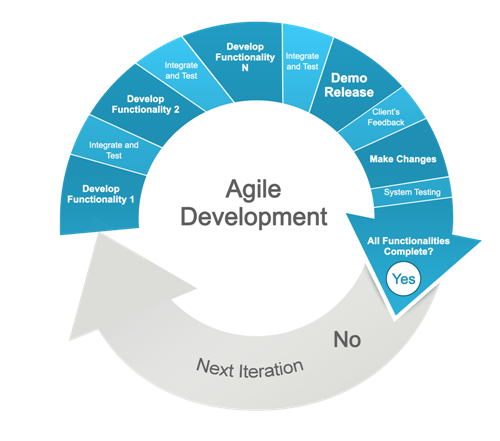
\includegraphics[height=7cm]{agile_development}
		\caption{Metodologia di sviluppo Agile}
	\end{center}
\end{figure}
\FloatBarrier

Le procedure, gli strumenti e le metriche adottate in The White Dog s.r.l. derivano da tre principali concetti di sviluppo Agile:

\subsubsection{DevOps}

Metodologia di sviluppo software che punta alla comunicazione, collaborazione e integrazione tra gli sviluppatori e addetti alle \textit{operations} dell'\textit{information technology}. DevOps vuole rispondere all'interdipendenza tra sviluppo software e IT \textit{operations}, puntando ad aiutare un'organizzazione a sviluppare in modo più rapido ed efficiente prodotti e servizi.

\label{DevOps}
\begin{figure}[ht]
	\begin{center}
		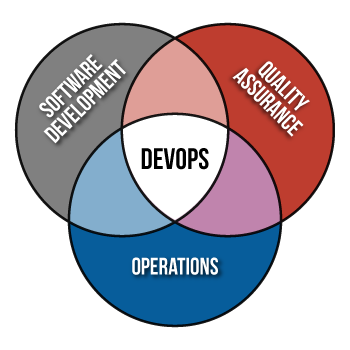
\includegraphics[scale=0.5]{devops-diagram}
		\caption{Competenze necessarie alla metodologia di sviluppo DevOps}
	\end{center}
\end{figure}
\FloatBarrier

In The White Dog s.r.l. questo principio è concretizzato dal fatto che ogni membro possiede sia le competenze di sviluppo, sia amministrative che di controllo della qualità, migliorando così di molto l'efficienza e l'agilità nello sviluppo del software e nel suo rilascio.

\subsubsection{Extreme Programming}

Metodologia di sviluppo software che enfatizza la scrittura di codice di qualità e la rapidità di risposta ai cambiamenti di requisiti. Prescrive lo sviluppo iterativo e incrementale soprattutto in brevi cicli di sviluppo. Suggerisce inoltre l'uso sistematico di \textit{unit testing} e \textit{refactoring}, vietando ai programmatori di sviluppare codice non strettamente necessario. Sostiene la chiarezza e la semplicità del codice, preferisce strutture gestionali non gerarchiche e dà molta importanza  alla comunicazione diretta e frequente fra sviluppatori e cliente e fra gli sviluppatori stessi. 

\label{Extreme Programming}
\begin{figure}[ht]
	\begin{center}
		
\includegraphics[scale=0.11]{extremeprogramming}
		\caption{Metodologia di sviluppo software Extreme Programming}
	\end{center}
\end{figure}
\FloatBarrier

Il \textit{team} di sviluppo di The White Dog s.r.l. fa ampio utilizzo di questa metodologia, spingendo molto sulla semplicità del codice prodotto, che dovrà poi essere utilizzato dagli sviluppatori Diana Corp., e sulla giornaliera comunicazione diretta tra gli sviluppatori e con il loro principale cliente, ovvero Diana Corp.. Questa comunicazione è facilitata dal fatto che The White Dog s.r.l. ha sede nello stesso stabilimento di Diana Corp..

\subsubsection{Kanban}

Metodologia atta al miglioramento dei processi per garantire una produzione \textit{Just in Time}. Essa prevede la presa di coscienza del proprio flusso di lavoro, visualizzandolo all'interno di una lavagna fisica, formata da tante colonne quante sono le fasi del processo produttivo.

\label{Kanban}
\begin{figure}[ht]
	\begin{center}
		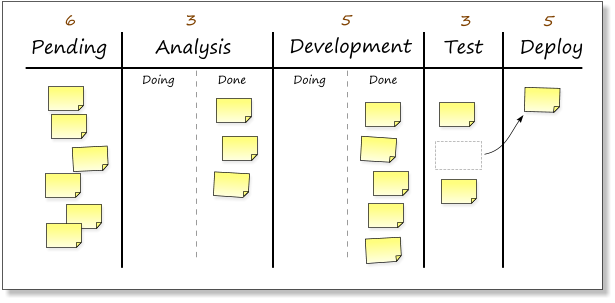
\includegraphics[scale=0.7]{kanban-board}
		\caption{Esempio di \textit{kanban board}}
	\end{center}
\end{figure}
\FloatBarrier

All'interno dello studio di The White Dog s.r.l. un interno muro bianco è dedicato alla \textit{kanban board}, dove il team prima di ogni sviluppo crea un nuovo \textit{workflow} per visualizzare le attività da fare e assegnarle agli sviluppatori.

\section{Strumenti e tecnologie}

All'interno di questa sezione parlerò degli strumenti e delle tecnologie adottate in azienda per lo sviluppo software.

\section{Ricerca e innovazione}

The White Dog s.r.l. nasce come reparto di ricerca e sviluppo di Diana Corp.. Essa dunque sperimenta e studia ogni giorno nuove tecnologie applicabili nel mondo del fashion e-commerce. \\
Ha a disposizione diversi dispositivi per la ricerca come \textit{smartphone} di ultima generazione, \textit{Smart TV}, \textit{smartwatch} e numerosi dispositivi per lo sviluppo AR e VR come \textit{Google Glass}, \textit{Oculus Rift Development Kit 2}, Google Cardboard e Leap Motion. Attraverso questi dispositivi l'azienda studia e sviluppa nuove modalità di interazione che l'utente finale può utilizzare nell'acquisto nei propri \textit{store} digitali.